% !TEX encoding = UTF-8 Unicode
%\chapter{QoS} 
\xchapter{QoS}{}
\label{cap:qos}
\acresetall
	QoS é o acrônimo para \textit{Quality of Service}, sendo um termo amplamente utilizado na literatura, mas em poucos artigos ele é definido. De acordo com \cite{GODERIS01}, QoS se refere a um serviço sendo oferecido onde um ou mais parâmetros de performance (isto é, vazão, atraso, perda e \textit{jitter}) podem ser quantificados. \cite{WANG01} define QoS como sendo "a capacidade de prover garantias de recursos e diferenciação de serviços em uma rede". Quando um canal de comunicação possui recursos reservados e algum nível de prioridade com relação a outros canais, podemos dizer que este canal possui uma QoS.	
	
\section{Arquiteturas de QoS}

	Diversas arquiteturas para prover QoS têm sido desenvolvidas nos últimos anos \cite{ACH96}. A motivação para a utilização de mecanismos de QoS, consequentemente para o desenvolvimento de arquiteturas de QoS, foi a necessidade de prover priorização e proteção a alguns fluxos de tráfegos \cite{GEBOSHIN03}, mas especificadamente aos tráfegos provindos das aplicações de tempo real, visto que estas necessitam de garantias temporais (previsibilidade). Este conjunto inclui os princípios que regem a construção de uma arquitetura genérica, a especificação da QoS que é necessária para capturar os requisitos da aplicação, e por último os mecanismos pelos quais os requisitos da aplicação serão atendidos. Basicamente os mecanismos podem ser divididos em dois tipos: provisão e controle/gerenciamento de QoS. Enquanto que o primeiro visa a reserva dos recursos, o outro visa a manutenção da QoS. Um dos componentes necessários para que esta manutenção ocorra corresponde ao monitoramento (não é o mesmo monitoramento do QoSP), pois é o mesmo que fornece o \textit{feedback} para saber se a QoS está sendo mantida. O módulo de monitoramento do QoSP deve se comunicar com o mecanismo de controle/gerenciamento das arquiteturas que estão sendo utilizadas no ambiente para conseguir obter a QoS que está sendo provida a um canal.
	
	Entre as diversas arquiteturas propostas na literatura, duas foram padronizadas pela IETF: os Serviços Integrados (\textit{Integrated Services} - \textit{IntServ}) e os Serviços Diferenciados (\textit{Differentiated Services} - \textit{Diffserv}). A seguir será apresentada de forma detalhada a arquitetura \textit{Diffserv}, visto que a mesma foi utilizada na implementação do QoSP.
	
\subsection{Diffserv}	

	Os Serviços Diferenciados \cite{BBCDWW98} baseiam-se na idéia de classes de comportamento, sendo que cada classe de comportamento define uma forma diferente de encaminhamento dos pacotes. Os pacotes pertencentes a diversos fluxos são agregados em classes e os pacotes da mesma classe são encaminhados na rede utilizando a mesma classe de comportamento. As reservas de recursos assim como o tratamento dado pelos roteadores (definido pelas classes de comportamento) aos pacotes é feito por classe, tornando o sistema escalável, visto que para um número grande de fluxos são configuradas poucas classes e, conseqüentemente, poucos estados são armazenados em cada roteador. Outra vantagem de se reservar recursos por classe é que raramente os recursos estarão ociosos, visto que frequentemente pelo menos um canal estará transmitindo algum dado. A maior parte do tráfego da Internet se comporta desta maneira, ou seja, nem todos os canais estarão transmitindo ao mesmo tempo.
	
	As classes de comportamento são chamadas de PHB (\textit{Per Hop Behavior}). As PHBs definem a forma como cada roteador irá encaminhar os pacotes para o outro roteador. Desta maneira, cada roteador deve possuir pré-configurado um conjunto de PHBs. Esta forma de encaminhamento se dá em termos dos recursos a serem utilizados e das propriedades do serviço que devem ser consideradas (como perdas, atraso, \textit{jitter}) \cite{GORENDER05}. Como podemos observar, a idéia do \textit{Diffserv} é oferecer níveis diferentes de serviço para os pacotes, ou seja, ele se baseia em um esquema de prioridade relativa \cite{XINI99}. O conjunto de fluxo de dados tratados da mesma forma (assinalados à mesma PHB) recebem o nome de Agregado de Comportamento (\textit{Behavior Aggregate}).
	
	Cada roteador identifica a classe de comportamento que será aplicada ao pacote através do \textit{DS Field}. Este corresponde a um campo do cabeçalho IP, e inclui seis bits que são utilizados pelo \textit{Diffserv} como um \textit{Codepoint} (\textit{DSCP}). Cada valor do \textit{DSCP} é mapeado para uma PHB em um roteador.

	Para que um determinado cliente possa receber Serviços Diferenciados do provedor de serviços (ISP), é necessário que seja estabelecido um Acordo de Ní­vel de Serviço (\textit{Service Level Agreement - SLA}) entre o cliente e o ISP. Este acordo informa o ní­vel de serviço assim como identifica as características do fluxo de dados que deverá receber o Serviço Diferenciado. O próprio cliente ou o ISP pode marcar o DSCP para configurar o serviço que será recebido pelo cliente.
	
	Um domí­nio \textit{Diffserv} (Figura \ref{fig:rede_diffserv}) é formado por roteadores (algumas literaturas chamam de nós) de dois tipos: roteadores de borda (também conhecidos como nós de fronteira) e de núcleo (também conhecidos como nós interiores) \cite{BBCDWW98}. Os roteadores de borda servem para interconectar domínios enquanto que os roteadores de núcleo apenas se conectam a outros roteadores do domínio. Os nós de fronteira implementam as funções de classificação, marcação, policiamento e condicionamento de tráfego, enquanto que os nós interiores apenas classificam, sendo que esta classificação é mais simples visto que ela é baseada apenas no DSCP, e encaminham pacotes. Esta estruturação da rede \textit{Diffserv} contribui para sua escalabilidade.
	
\begin{figure}
\centering
%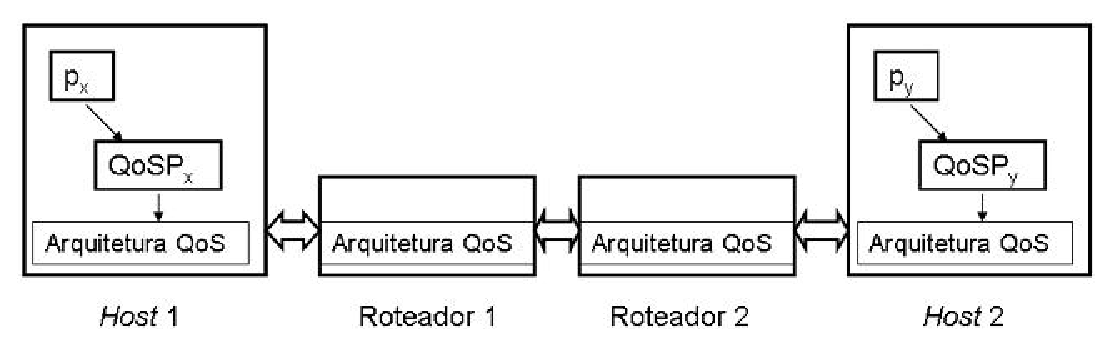
\includegraphics[width=0.3\textwidth]{qosp}
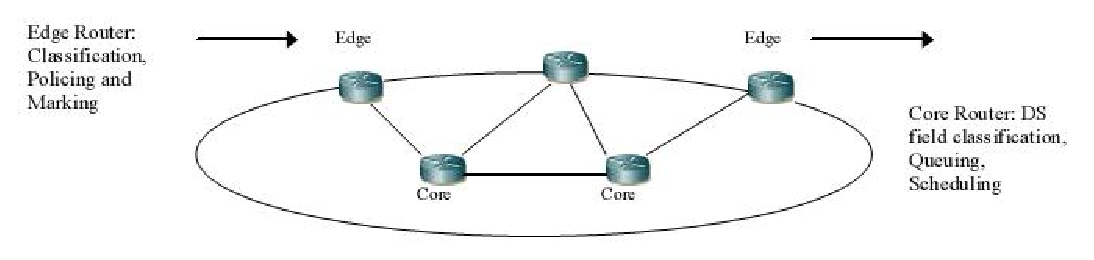
\includegraphics[scale=0.7]{rede_diffserv}
\caption{Rede Diffserv \cite{KFF03}}
\label{fig:rede_diffserv}
\end{figure}	
	
	Existem quatro PHBs padronizadas pelo IETF mas, para que o QoSP funcione (visto que os canais gerenciados pelo QoSP necessitam de dois tipos de serviços), apenas duas PHBs são necessárias e, consequentemente, serão abordadas: Padrão e o Serviço Expresso. Estes serviços caracterizam os níveis extremos de garantias, visto que enquanto o primeiro não possui garantia nenhuma, o segundo possui garantias suficientes para que o pacote sofra o menor atraso possível nos roteadores. 
	
\subsubsection{Padrão}

	A PHB Padrão especifica que os pacotes deverão receber o serviço melhor esforço (\textit{best-effort}). Neste caso, os pacotes que possuem tal serviço não têm prioridade e não possuem garantias de recursos. Este serviço será utilizado pelos canais de comunicação \textit{untimely}, que serão descritos no capítulo \ref{cap:qos_provider}.

\subsubsection{Serviço Expresso}	

	O Serviço Expresso (\textit{Expedited Forwarding} - EF), sendo também chamado em algumas bibliografias por serviço \textit{Premium}, basicamente visa garantir baixa latência e \textit{jitter}, além de uma largura de banda garantida. De forma intuitiva, para que o roteador forneça o Serviço Expresso basta que a taxa de saída dos pacotes seja maior ou igual a uma taxa de entrada previamente configurada \cite{BBCDWW98}. Com isso, caso os fluxos de dados não excedam a taxa de transmissão previamente configurada, praticamente estes pacotes não permanecerão em fila. Este serviço será utilizado pelos canais de comunicação \textit{timely}, descritos no capítulo \ref{cap:qos_provider}.
\section{Sistemas de monitoramento}	
	
	A monitoração de QoS é um mecanismo utilizado por outros componentes para obter um \textit{feedback} sobre o estado atual da QoS, para que medidas possam ser tomadas baseado neste \textit{feedback}. A reserva dos recursos não é suficiente para se obter QoS, visto que a degradação da mesma é inevitável \cite{JTK00}. De acordo com \cite{ACH96}, a monitoração da QoS é um componente essencial para o mecanismo de gerenciamento. Ela é responsável por descobrir o nível de QoS que está sendo provido por cada componente do serviço de comunicação para que se possa então verificar uma eventual degradação da qualidade de serviço fornecida. Quando a degradação é detectada, esta deve ser informada à aplicação e, neste caso, a aplicação poderá reagir de maneira adequada à perda da QoS, assumindo a perda no nível do serviço ou tentando renegociar uma nova QoS para o canal de comunicação. De acordo com \cite{ACH96}, o mecanismo de gerenciamento deve tentar resolver a perda da QoS antes de informar à aplicação sobre a degradação. O módulo de monitoração do QoSP deve apenas verificar e informar a QoS que está sendo provida ao canal, não sendo necessário resolver uma possível perda.
	
	Mesmo o módulo de monitoração do QoSP não sendo um componente de um arquitetura de QoS, ele se comporta como um para o QoSP, visto que ele é responsável por descobrir o nível de QoS que está sendo provido por cada arquitetura de QoS utilizada. Sendo assim, é importante que modelos e princípios de um sistema de monitoramento sejam utilizados.
	
\subsection{Princípios} %\label{subsub: principios}

	De acordo com \cite{ATIPPEB02}, a escalabilidade nas redes IP com QoS está ligada a três fatores: tamanho da topologia da rede, número e granularidade das classes de serviço suportadas na rede e o número de clientes que utilizam os serviços. Um sistema de monitoramento é considerado escalável se o mesmo consegue monitorar de forma eficiente uma grande rede com vários serviços e uma grande quantidade de clientes. Além disso, o sistema de monitoramento deve realizar as seguintes tarefas: coletar, agregar e analisar dados, além de prover um \textit{feedback} sobre a QoS atual. Ainda de acordo com \cite{ATIPPEB02}, para que o sistema de monitoramento seja escalável, é preciso que o mesmo siga os  princípios descritos abaixo.

\begin{enumerate}

\item Definir granularidade do processo de monitoramento
	
	Os algoritmos de monitoramento devem operar no nível do agregado e não no nível do pacote, visto que coletar dados no nível de pacote é  extremamente custoso e não escalável. No Diffserv, estas estatísticas seriam coletadas por PHB.
	
\item Distribuir o sistema coletor de dados
	
	Para que o sistema coletor de dados não gere um \textit{overhead} grande na rede, ele deve ser distribuído, preferencialmente um agente coletor por cada roteador e o mais próximo possível do mesmo.
	
\item Minimizar o \textit{overhead} da transmissão das medições através do processamento dos dados brutos próximo às fontes

	Assim como o sistema de coleta de dados, o processamento e sumarização dos dados também deve ser distribuído para que o sistema seja escalável. Além do mais, o sistema de monitoração pode adotar a política de notificação de eventos quando certos limiares são ultrapassados. A notificação é utilizada para evitar a sobrecarga da rede com interações desnecessárias entre componentes requisitando informações de monitoramento.
	
\item Utilizar medições por agregado em combinação com medições por canal

	Vários fluxos de dados possuem requisitos diferentes e por isso devem ser monitorados de forma diferente. Mas monitorar os canais de forma diferente torna o sistema complexo. Além disso, vários canais de comunicação passam pelo mesmo caminho na rede, conseqüentemente as medições feitas para um canal podem ser utilizadas para os outros canais, colaborando para a escalabilidade do sistema. Dessa forma deve-se optar por uma medição por agregado e, quando isso não for possível devido a requisitos diferentes ou caminhos diferentes pelos quais os canais passam, utiliza-se a medição por canal.

\end{enumerate}	

\subsection{Modelo de monitoramento de QoS} %\label{subsub: modelo}

	De acordo com \cite{JTK00}, os mecanismos de monitoramento podem ser divididos em duas categorias, baseado na informação de QoS que pode ser obtida através deles: monitoração de QoS fim-a-fim e a monitoração distribuída de QoS. Na monitoração fim-a-fim, apenas a QoS fim-a-fim de um canal de comunicação é monitorada. Neste caso, a degradação da QoS consegue ser detectada, mas o componente que está causando tal degradação não. Na abordagem distribuída, a QoS que está sendo provida por cada elemento ao longo do canal é monitorada, permitindo saber quais são os elementos que estão causando a degradação. Enquanto que na abordagem fim-a-fim as informações de monitoramento são coletadas nos sistemas fins, ou seja nos \textit{hosts}, na abordagem distribuída estas informações são colhidas dos monitores relevantes, ou seja, dos elementos que estão monitorando os roteadores que fazem parte de um determinado canal. A abordagem distribuída além de contribuir para a escalabilidade permite que medidas de correção sejam tomadas, visto que o problema pode ser isolado. O modelo de monitoramento adotado em \cite{JTK00} (Figura \ref{fig:modelo}) é semelhante ao modelo tradicional de sistema de monitoramento apresentado em \cite{STALL96}, sendo dividido nos seguintes componentes:

\begin{figure}
\centering
%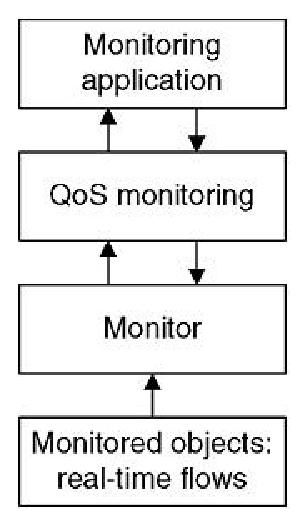
\includegraphics[width=0.3\textwidth]{modelo}
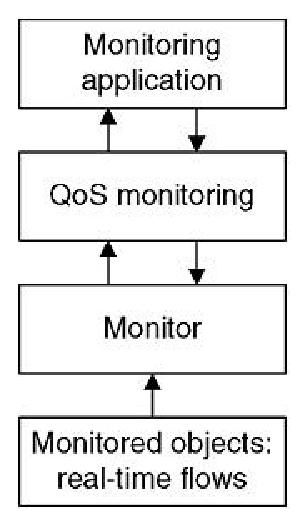
\includegraphics[scale=0.7]{modelo}
\caption{Modelo de monitoramento de QoS \cite{JTK00}}
\label{fig:modelo}
\end{figure}

\textbf{Monitoring application:} Este componente provê a interface do sistema de monitoramento com o usuário (ou um outro cliente interessado na informação de monitoramento, como o detector de defeitos). Recolhe (agrega) as informações colhidas pelos \textit{monitores} (o componente \textit{Monitor}), analisa estas informações e provê os resultados da análise para o usuário. Estes resultados correspondem à QoS que está sendo provida ao canal de comunicação.

\textbf{QoS monitoring:} Este componente não existe no modelo tradicional. Este componente provê mecanismos para permitir que \textit{Monitoring application} recupere a informação dos \textit{monitores} relevantes, ou seja, aqueles que monitoram os roteadores que fazem parte do canal de comunicação em questão. A QoS do canal é derivada a partir das informações capturadas pelos \textit{monitores}.

\textbf{Monitor:} É responsável por colher e armazenar as informações provenientes dos roteadores. Estas informações são comunicadas ao \textit{Monitoring application}.

\textbf{Monitored objects:} Estes objetos correspondem aos atributos e atividades que devem ser monitoradas na rede. Estes objetos equivalem a contadores dos fluxos de tempo real monitorados.

	Como foi explicado anteriormente, o sistema de monitoramento desempenha um conjunto de funções básicas. Estas funções podem ser mapeadas para o modelo descrito acima da seguinte maneira: a função de coletar os dados fica à cargo de \textit{Monitor}, enquanto que as funções de agregação e análise dos dados, além do \textit{feedback} provido contendo a QoS do canal são de responsabilidade de \textit{Monitoring application}.

\subsection{Colhendo informações de QoS}
	Os sistemas de monitoramento precisam se comunicar com os elementos de rede (como os roteadores) para colher informações de QoS. Algumas vezes essas interações são necessárias para que informações mais detalhadas sobre o estado da QoS que está sendo provida pelos elementos sejam capturadas. O protocolo SNMP é utilizado para gerenciar os elementos de rede, sendo descrito a seguir.
	
\subsubsection{SNMP}

	O SNMP (\textit{Simple Network Management Protocol}) foi concebido para monitorar os nós (\textit{hosts}, \textit{switches}, roteadores, etc) na Internet \cite{CFSD90}. Ele é formado por três componentes: o agente, o gerente (conhecido também como sistema de gerenciamento) e os dispositivos gerenciados (\textit{hosts}, roteadores, etc). Os agentes são elementos de software instalados nos dispositivos gerenciados cuja função principal é enviar informações relativas aos dispositivos para os gerentes.
	
	Todas as informações gerenciáveis são definidas através de variáveis nos dispositivos gerenciados. Estas variáveis contém valores que são lidos (quando o gerente solicita ao agente uma operação de leitura) ou atualizados (quando o gerente solicita ao agente uma operação de escrita). Essas informações gerenciáveis podem ser: número IP, quantidade de pacotes descartados, tamanho de filas, largura de banda reservada para classes, dentre inúmeras outras. Estas variáveis são estruturadas hierarquicamente (como numa árvore) na MIB.
	
	 Uma \textit{Management Information Base} (MIB) contém a definição dos objetos gerenciáveis. Os objetos gerenciáveis são conhecidos como objetos MIB, e são formados por várias instâncias de objeto. Por exemplo, um número de interface em um roteador é um objeto MIB e, sabendo que um roteador é formado por várias interfaces, o número de uma interface específica seria uma instância de objeto. Cada instância de objeto é identificada por um OID (\textit{object identifier}). Cada instância de objeto corresponde à uma variável citada anteriormente.